\subsection{Algoritmo} \label{sec:algo}
Pela descrição do problema, para definir os tutores de cada aluno o sistema
utiliza uma árvore binária de busca, em que o pai do aluno na árvore é seu
tutor. Entretanto o custo da inserção seria probitivo se utilizássemos a mesma
estrutura para encontrar os tutores, que no pior caso, teríamos uma árvore
binária degenerada com complexidade de inserção O(n). Observa-se que a árvore binária de busca define uma sequência de matrículas
relacionado a um determinado percurso. Nossa solução
(algoritmo~\ref{alg:parent}) propõe modelar a mesma
sequência, entretanto utilizando uma árvore binária balanceada auxiliar
para calcular os pais e altura dos alunos em realação a árvore binária de busca
original.

\begin{algorithm}[]
  \small
  \caption{Cálcula o pai (tutor) de cada matrícula, modelando a sequência
    \textit{inorder} de uma árvore binária de busca utilizando uma árvore binárea
    balanceada.}\label{alg:parent}
  \begin{algorithmic}[1]
    \Require $mat[N]$ vetor de matrículas de tamanho $N$; $parent$ tabela \textit{hash}.
    \Procedure{Parents}{$mat[N], parent$}% \Comment{Vetor de matrículas de tamanho $N$.}
    % \State $keys[N] \gets 0$\Comment{Vetor de chaves com tamanho $N$.}
    \State $order \gets$ \Call{SplayTree}{ }
    % \State $parent \gets$ \Call{HashTable}{N}
    \State $level \gets$ \Call{HashTable}{N}

    \Statex
    \For{$i \gets 0, N$}
    % \State $keys[i] \gets mat[i]$

    \If{$order \neq \emptyset$}
    \State $upper \gets$ \Call{LowerBound}{$order, mat[i]$}
    \Statex
    \If{$upper$ not found}
    % \State // Matrículas são menores que $mat[i]$. Sequência ord.: $\ldots
    % W X$
    % \Statex
    \State $w \gets$ \Call{Max}{$order$} \Comment{Maior elemento de $order$.}
    \State $l \gets$ \Call{LookUp}{$level, w+1$} \Comment{$l = level[w+1]$}
    \State \Call{Insert}{$parent, mat[i], w$} \Comment{$parent[mat[i]] = w$}
    \State \Call{Insert}{$level, mat[i], l$}
    \Statex
    \ElsIf{$upper = $ \Call{Min}{$order$}} \Comment{Menor elemento de $order$}
    % \State // Matrículas são maiores que $x$. Sequência ord.: $X W
    % \ldots$
    % \State $w \gets$ \Call{Min}{$order$}
    \State $l \gets$ \Call{LookUp}{$level, upper+1$}
    \State \Call{Insert}{$parent, mat[i],upper$}
    \State \Call{Insert}{$level, mat[i],l$}
    \Statex
    \Else
    \State $lower \gets$ \Call{Previous}{$order, upper$} \Comment{Elemento anterior em $order$}
    \Statex
    % \State // $lower$ e $upper$ estão no meio. Sequência ord.: $\ldots~ L ~
    % X ~ U ~\ldots$
    % \Statex
    % \State // $upper$ é o pai? $upper$ está na subárvore de $lower$?
    \If{\Call{LookUp}{$level, upper$} $>$ \Call{LookUp}{$level, lower$}}
    \State $l \gets$ \Call{LookUp}{$level, upper$}
    \State \Call{Insert}{$parent, mat[i], upper$}
    \State \Call{Insert}{$level, mat[i], l+1$}
    \Statex
    \Else
    % \State // $lower$ é o pai? $lower$ está na subárvore de $upper$?
    \State $l \gets$ \Call{LookUp}{$level, lower$}
    \State \Call{Insert}{$parent, mat[i], lower$}
    \State \Call{Insert}{$level, mat[i], l+1$}
    \EndIf
    \EndIf \Comment{$upper$ not found}
    \EndIf \Comment{$order \neq \emptyset$}
    \Statex
    \State \Call{Insert}{$order, mat[i]$}
    \State $i \gets i + 1$
    
    \EndFor
    \EndProcedure
  \end{algorithmic}
\end{algorithm}

O algoritmo recebe uma lista de matrículas ($mat$) e uma tabela ($parent$) associando alunos e
tutores vazia. Inicializamos definindo uma \textit{splay tree} ($order$), aonde
serão feitas as inserções, e outra tabela ($level$) associando a matrícula à
altura na árvore original, linhas 2 e 3. Após a inicialização, percorremos todos
os alunos (linha 4), simulando o percurso original (linhas 5--34) e finalmente
inserimos na árvore balanceada (linha 35). Entre as linhas 6--34 queremos
encontrar qual posição da sequência a matrícula $i$ ($mat[i]$) encaixará,
para isso procuramos (linha 6) pela menor matrícula ($upper$) tal que seja maior
ou igual à matrícula $i$ ($mat[i]$) na árvore $order$. Caso a matrícula ($upper$) não
exista, podemos concluir que nossa sequência terá o seguinte formato após inserção: $(\ldots,
w,mat[i])$, ou seja $m[i]$ é maior que todas as matrículas na árvore binária de
busca e filho de $w$. Assim obtemos o maior elemento da sequência ($w$ linha
9) e a altura ($l$) na qual $m[i]$ seria inserido na árvore (linha 10),
finalmente atualizamos as tabelas de pais e alturas com os novos dados de $m[i]$
(linhas 11--12). Caso a matrícula exista ($upper$) ela pode ser o primeiro
elemento da sequência (linhas 13--18), isto é a menor matrícula, ou estar em qualquer posição no
meio da sequência (linhas 19--33). Se $upper$ for o menor elemento da árvore
$order$, a sequência terá formato: $(mat[i], w, \ldots)$, ou seja, $mat[i]$ é a
menor matrícula na árvore original com pai $upper$. Analogamente, obtemos a altura ($l$) na qual
$m[i]$ seria inserido e atualizamos a tabela de pais e nível (linhas 15--17).
Para o último caso teríamos sequência de formato: $(\ldots, lower, mat[i],
upper, \ldots)$, em que $lower$ é a matrícula anterior a $upper$ em $order$
(linha 19).
\begin{figure}[!htb]
  \centering
  % dot -Gdpi=300 -Tpng test1.dot > test1.png
  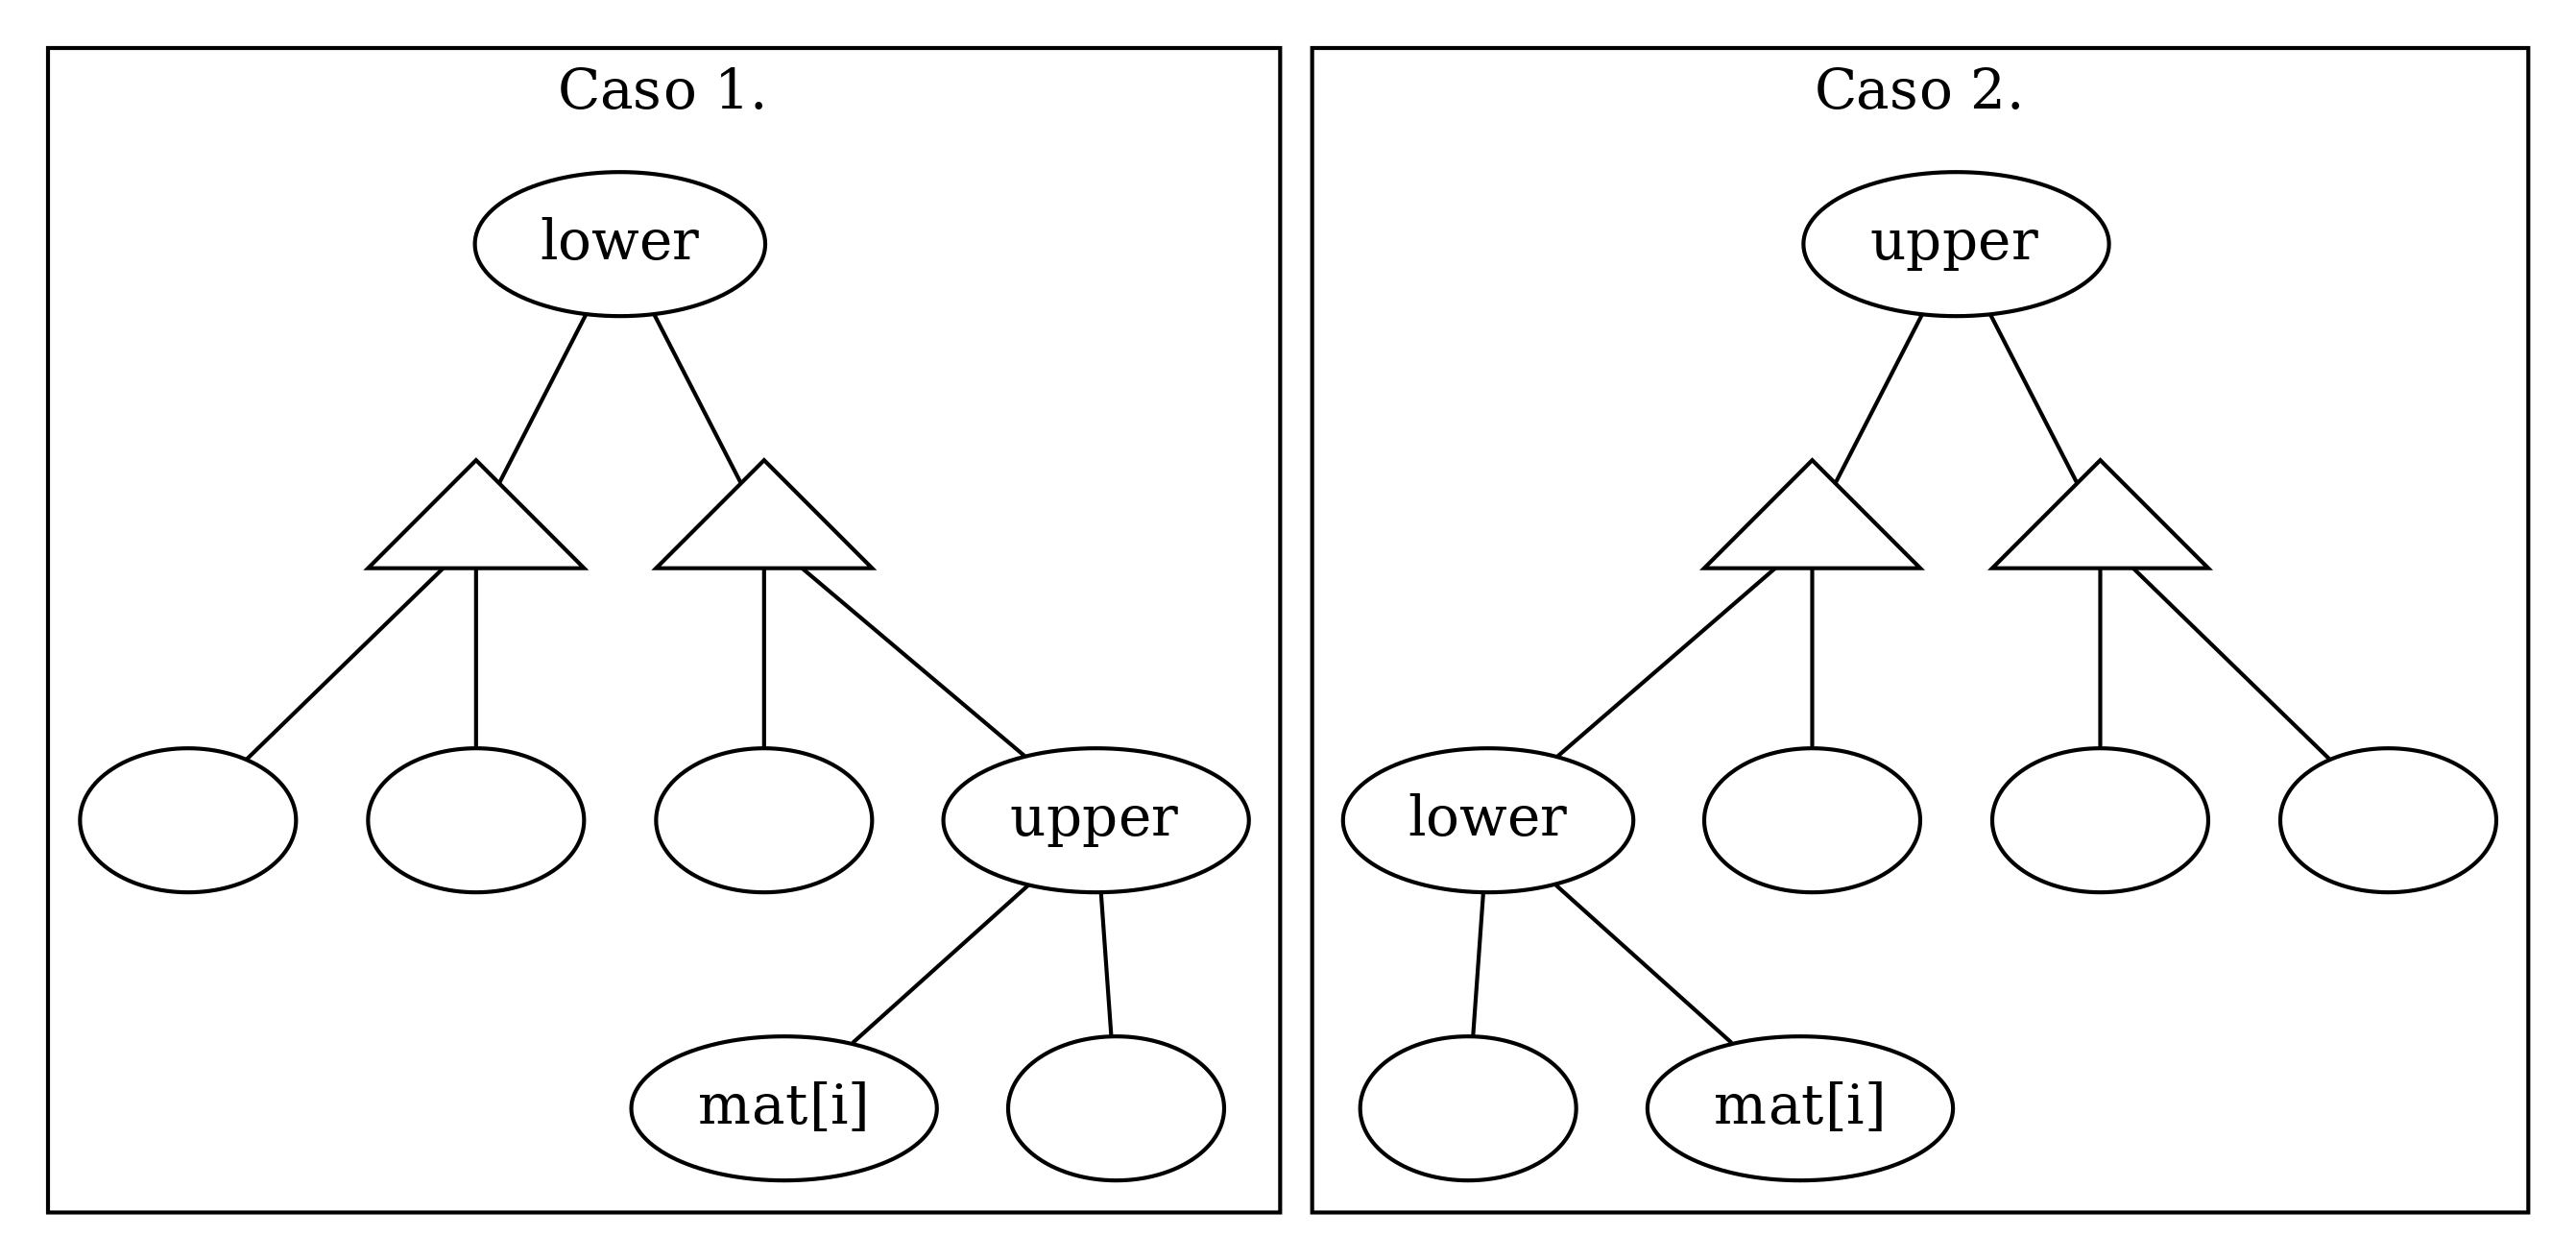
\includegraphics[width=0.7\linewidth]{lxu.png}
  \caption{Algo}
  \label{fig:lxu}
\end{figure}
Neste paço temos duas configurações possíveis, como pode ser visto
na figura~\ref{fig:lxu}, portanto precisamos determinar quem está na subárvore
de quem (linha 22) para escolher a configuração correta: se $lower$ está na
subárvore de $upper$ então $upper$ é pai de $mat[i]$ (linhas 23--25), caso
contrário, $lower$ é pai de $mat[i]$ (linhas 28--30). Ao final do algoritmo a
tabela $parent$ possui os tutores de cada aluno.

\subsubsection{Análise da complexidade}
